\documentclass[a4paper,10pt,twocolumn]{ltjarticle}
\usepackage{kaitoushu}

\pgfplotsset{
  myaxis/.style={
    axis lines=middle,
    xlabel={$x$}, ylabel={$y$},
    every axis x label/.style={at={(ticklabel* cs:1)},anchor=west},
    every axis y label/.style={at={(ticklabel* cs:1)},anchor=south},
    tick label style={font=\scriptsize},
    label style={font=\small},
    width=5.5cm, height=5cm,
    grid=none,
    samples=200,
  }
}

\begin{document}

\problemrange{4章：指数関数と対数関数 — 練習問題2・A (p.123)}



\mondai{1}{次の等式を満たす $x$ の値を求めよ．}
\kotae{
$\log_{a}M=p \Leftrightarrow a^{p}=M$ を使う．

\textbf{(1)} $\log_{3}x=3 \Rightarrow x=3^{3}=27$

\textbf{(2)} $\log_{1/3}x=-1 \Rightarrow x=\left(\dfrac{1}{3}\right)^{-1}=3$

\textbf{(3)} $\log_{8}x=\dfrac{2}{3} \Rightarrow x=8^{2/3}=(2^{3})^{2/3}=4$

\textbf{(4)} $\log_{x}16=4 \Rightarrow x^{4}=16=2^{4}$．$x>0,\;x\neq1$ より $x=2$

\textbf{(5)} $\log_{x}\sqrt[4]{4}=\dfrac{1}{2} \Rightarrow x^{1/2}=4^{1/4}=2^{1/2}$．$\therefore x=2$

\textbf{(6)} $\log_{\sqrt{3}}\dfrac{1}{27}=x$

$(\sqrt{3})^{x}=3^{-3} \Rightarrow 3^{x/2}=3^{-3} \Rightarrow x=-6$
}

\mondai{2}{次の式を簡単にせよ．}
\kotae{
\textbf{(1)} $\log_{2}10+\log_{2}20-2\log_{2}5$

$=\log_{2}\dfrac{10\cdot20}{5^{2}}=\log_{2}\dfrac{200}{25}=\log_{2}8=3$

\textbf{(2)} $\dfrac{1}{2}\log_{6}\dfrac{4}{9}+\log_{6}\dfrac{1}{4}$

$=\log_{6}\dfrac{2}{3}+\log_{6}\dfrac{1}{4}=\log_{6}\dfrac{1}{6}=-1$

\textbf{(3)} $(\log_{3}25)(\log_{5}9)(\log_{5}8)$

常用対数 $\log$ で書き換え：
\[
\log_{3}25=\dfrac{2\log5}{\log3},\;\log_{5}9=\dfrac{2\log3}{\log5}
\]

前2つの積：
\[
\dfrac{2\log5}{\log3}\cdot\dfrac{2\log3}{\log5}=4
\]

残り：$\log_{5}8=3\log_{5}2$ を掛けて

$\therefore 4\cdot3\log_{5}2=12\log_{5}2$
}

\mondai{3}{$\log_{2}3=m$ のとき，$\log_{6}9$ を $m$ で表せ．}
\kotae{
\[
\log_{6}9=\dfrac{\log9}{\log6}=\dfrac{2\log3}{\log2+\log3}
\]

分子分母を $\log2$ で割る：
\[
=\dfrac{2\cdot\frac{\log3}{\log2}}{1+\frac{\log3}{\log2}}=\dfrac{2m}{1+m}
\]
}

\mondai{4}{次の数を大きいものから順に並べよ．}
\kotae{
\textbf{(1)} $\log_{3}4,\;2,\;\log_{3}\sqrt{45},\;\dfrac{1}{2}\log_{3}50$

$\log_{3}\Box$ の形に統一：
\[
2=\log_{3}9,\;\dfrac{1}{2}\log_{3}50=\log_{3}\sqrt{50}
\]

真数比較：$4<\sqrt{45}\approx6.71<\sqrt{50}\approx7.07<9$．底 $3>1$ は単調増加．

$\therefore 2>\dfrac{1}{2}\log_{3}50>\log_{3}\sqrt{45}>\log_{3}4$

\textbf{(2)} $\log_{0.5}\sqrt{3},\;\log_{0.5}\sqrt[3]{2},\;\log_{0.5}\sqrt[5]{6}$

底 $0.5<1$ なので単調減少．真数が小さいほど値は大きい：
\[
\sqrt[3]{2}\approx1.26<\sqrt[5]{6}\approx1.43<\sqrt{3}\approx1.73
\]

$\therefore \log_{0.5}\sqrt[3]{2}>\log_{0.5}\sqrt[5]{6}>\log_{0.5}\sqrt{3}$
}

\mondai{5}{次の関数のグラフをかけ．}
\kotae{
\textbf{(1)} $y=\log_{2}(x+2)$：$y=\log_{2}x$ を左に $2$ 平行移動．定義域 $x>-2$，漸近線 $x=-2$，$(0,1),(-1,0)$ を通る．

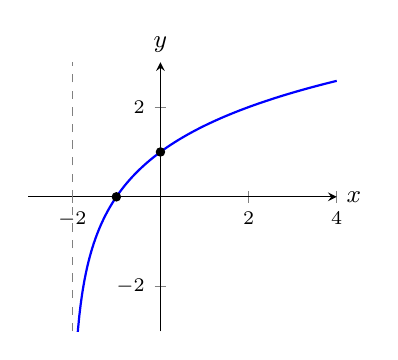
\begin{tikzpicture}
\begin{axis}[myaxis, xmin=-3,xmax=4,ymin=-3,ymax=3]
\addplot[thick,blue,domain=-1.9:4]{ln(x+2)/ln(2)};
\addplot[dashed,gray] coordinates {(-2,-3)(-2,3)};
\addplot[only marks,mark=*,mark size=1.5pt] coordinates {(-1,0)(0,1)};
\end{axis}
\end{tikzpicture}

\textbf{(2)} $y=-\log_{3}x$：$y=\log_{3}x$ を $x$ 軸に関して折り返し．定義域 $x>0$，$(1,0),(3,-1),(1/3,1)$ を通る．

\begin{tikzpicture}
\begin{axis}[myaxis, xmin=-1,xmax=5,ymin=-3,ymax=3]
\addplot[thick,blue,domain=0.1:5]{-ln(x)/ln(3)};
\addplot[only marks,mark=*,mark size=1.5pt] coordinates {(1,0)(3,-1)};
\end{axis}
\end{tikzpicture}

\textbf{(3)} $y=\log_{2}(2-x)$：$y=\log_{2}(-x)$ を右に $2$ 平行移動．定義域 $x<2$，漸近線 $x=2$，$(1,0),(0,1)$ を通る．

\begin{tikzpicture}
\begin{axis}[myaxis, xmin=-4,xmax=3,ymin=-3,ymax=3]
\addplot[thick,blue,domain=-4:1.9]{ln(2-x)/ln(2)};
\addplot[dashed,gray] coordinates {(2,-3)(2,3)};
\addplot[only marks,mark=*,mark size=1.5pt] coordinates {(1,0)(0,1)};
\end{axis}
\end{tikzpicture}
}

\mondai{6}{次の方程式を解け．
\[
\log_{4}(x-1)+\log_{4}(x-3)=\log_{4}(13-x)
\]}
\kotae{
真数条件：$x-1>0,\;x-3>0,\;13-x>0$ より $3<x<13$．

対数の和を積に：
\[
\log_{4}(x-1)(x-3)=\log_{4}(13-x)
\]
\[
(x-1)(x-3)=13-x
\]
\[
x^{2}-4x+3=13-x
\]
\[
x^{2}-3x-10=0 \Rightarrow (x-5)(x+2)=0
\]

$3<x<13$ より $x=5$（$x=-2$ は不適）．

$\therefore x=5$
}

\mondai{7}{次の不等式を解け．}
\kotae{
\textbf{(1)} $\log_{4}(1-3x)\geqq2$

真数条件：$1-3x>0 \Rightarrow x<\dfrac{1}{3}$．

底 $4>1$ より $1-3x\geqq4^{2}=16$．
$-3x\geqq15 \Rightarrow x\leqq-5$．

$\therefore x\leqq-5$

\textbf{(2)} $\log_{4}(1-3x)\leqq2$

真数条件：$x<\dfrac{1}{3}$．

底 $4>1$ より $0<1-3x\leqq16$．
$1-3x\leqq16 \Rightarrow x\geqq-5$．

$\therefore -5\leqq x<\dfrac{1}{3}$
}

\mondai{8}{光がある種のガラス板を1枚透過するごとに，その明るさが $9\%$ 失われるという．このガラス板を何枚重ねると，透過した光の明るさがはじめの4割以下になるか．ただし，$\log_{10}2=0.3010,\;\log_{10}7=0.8451$ とする．}
\kotae{
1枚透過で $0.91$ 倍．$n$ 枚重ねた後の割合は $0.91^{n}$．

条件：$0.91^{n}\leqq0.4$

両辺の常用対数をとる：
\[
n\log_{10}0.91\leqq\log_{10}0.4
\]

各対数を計算：
\[
\log_{10}0.4=\log_{10}\dfrac{4}{10}=2\log_{10}2-1
\]
\[
=2(0.3010)-1=-0.3980
\]
\[
\log_{10}0.91\approx-0.0410
\]
（$\log_{10}91=\log_{10}(7\cdot13)$ 等から近似）

$\log_{10}0.91<0$ なので両辺を割ると不等号反転：
\[
n\geqq\dfrac{-0.3980}{-0.0410}\approx9.70
\]

$n$ は整数なので $n\geqq10$．

$\therefore 10$ 枚以上
}

\end{document}
